\structure{ОСНОВНАЯ~ЧАСТЬ}

В основной части исследовательской работы проводится комплексный анализ,
проектирование и реализация распределённой вычислительной системы. Работа
начинается с анализа предметной области, где рассматриваются подходы к
построению распределённых вычислительных систем, включая историю их развития и
архитектурные особенности. Далее исследуются проблемы согласованности и
отказоустойчивости, что приводит к обоснованию выбора алгоритма консенсуса Raft
для обеспечения надёжности системы.

Подробно изучается алгоритм Raft, уделяя особое внимание роли лидера и
механизмам работы в различных сценариях отказов. На основе проведённого анализа
проектируется архитектура системы, включающая общую структуру, роли узлов,
потоки управления и данные, а также вопросы отказоустойчивости и
масштабирования. Рассматриваются архитектурные решения для Raft-узлов,
клиентской части и вычислительных узлов.

Затем описывается практическая реализация системы с обоснованием выбора
технологий и инструментов. Детализируется реализация ключевых компонентов:
Raft-узла с механизмом снимков данных, серверного модуля, менеджера
заданий и вычислительных узлов. Завершает основную часть ручное тестирование
системы, включающее проверку отказоустойчивости, инициализации клиентских
приложений, подключения вычислительных узлов, выполнения заданий, нагрузочного
тестирования и работы с большими объёмами данных.

\section{Анализ предметной области}

В этой части рассматриваются современные подходы к построению распределённых
систем и анализируются их ключевые характеристики: масштабируемость,
отказоустойчивость и согласованность. Подробно описываются типичные проблемы,
возникающие при проектировании систем, работающих на множестве узлов, включая
сетевые задержки, отказы оборудования и необходимость достижения единого
состояния. Отдельное внимание уделяется понятию консенсуса и роли алгоритмов
консенсуса в обеспечении корректной работы распределённых систем.

\subsection{Подходы к построению распределённых вычислительных систем}

\subsubsection{История развития распределенных вычислительных систем}

Область распределённых вычислительных систем в последние десятилетия
характеризуется высокой динамикой развития концепций и подходов. За
сравнительно короткий период появилось множество парадигм построения
распределённых вычислений, каждая из которых оказывала значительное влияние на
индустрию, но со временем уступала место новым методам. Часто идеи не исчезают
полностью, а возвращаются в обновлённом виде, что приводит к постоянному
сочетанию устоявшихся принципов с современными инженерными практиками.

В 1990-х годах можно выделить два доминирующих подхода к созданию
распределённых систем. Первый был связан с развитием Всемирной паутины, которая
рассматривалась как глобальное информационное пространство, ориентированное на
взаимодействие людей. Второй подход основывался на технологиях распределённых
объектов, таких как CORBA \cite{siegel1998corba} и DCOM\cite{microsoftDCOM},
которые позволяли строить распределённые приложения, имитирующие локальные
среды выполнения и предоставляющие прозрачный доступ к удалённым ресурсам.
Несмотря на масштабное развитие этих технологий, Веб оставался в основном
средством потребления информации, а распределённые объекты становились всё
более сложными и трудоёмкими в использовании.

С начала 2000-х годов начался активный рост новых технологий и платформ
промежуточного программного обеспечения. Широкое распространение получили
одноранговые (peer-to-peer) сети, позволившие пользователям не только получать,
но и предоставлять ресурсы. Параллельно развивались грид-технологии,
ориентированные на объединение крупных вычислительных и хранительных комплексов
для совместного решения научных и прикладных задач. Грид-системы впервые
предложили концепцию «вычислений по требованию», по аналогии с доступом к
коммунальным услугам, что стало важным этапом на пути к современным облачным
вычислениям.

За последние два десятилетия архитектура программных систем сместилась от
монолитных решений к распределённым и облачным подходам, ориентированным на
горизонтальное масштабирование, географическое распределение нагрузки и высокую
доступность сервисов. Широкое распространение получили микросервисные и
событийно-ориентированные архитектуры, а также шаблоны репликации и разделения
данных, позволяющие изолировать сбои и наращивать производительность за счёт
параллелизма.

\subsubsection{Архитектура распределенных вычислительных систем}

Эндрю Таненбаум предложил следующее определение распределенных вычилительных
систем \cite{tanenbaum_distributed_systems}:

«Распределенная вычислительная система (РВС) – это набор соединенных каналами
связи независимых компьютеров, которые с точки зрения пользователя некоторого
программного обеспечения выглядят единым целым».

Данное определение подчёркивает два ключевых аспекта: самостоятельность
функционирования узлов распределённой вычислительной системы и её восприятие
пользователем как единого целого. При этом центральную роль в обеспечении
согласованной работы всех компонентов играет программное обеспечение,
выступающее связующим элементом системы.

К числу основных свойств РВС относят:
\begin{itemize}
    \item поддержку работы с разнородными устройствами и платформами, включая
        различные операционные системы и оборудование разных производителей;
    \item возможность масштабирования и наращивания ресурсов без существенных
        изменений архитектуры;
    \item обеспечение непрерывного доступа к ресурсам даже при временной
        недоступности отдельных узлов;
    \item сокрытие от пользователя технических деталей взаимодействия
        компонентов.
\end{itemize}

Если распределённая среда состоит из узлов с различными аппаратными и
программными конфигурациями, она называется гетерогенной. Для объединения
подобных узлов в единую систему стек программного обеспечения РВС традиционно
делят на два уровня. Верхний уровень составляют распределённые приложения,
реализующие прикладные функции. Они опираются на нижний уровень — промежуточное
программное обеспечение (middleware), которое взаимодействует с системными и
сетевыми сервисами, обеспечивая прозрачность работы приложений и единообразие
взаимодействия внутри кластера. Пример архитектуры приведен на рис.
\ref{fig:distributed-architecture}.

\begin{figure}
  \centering
  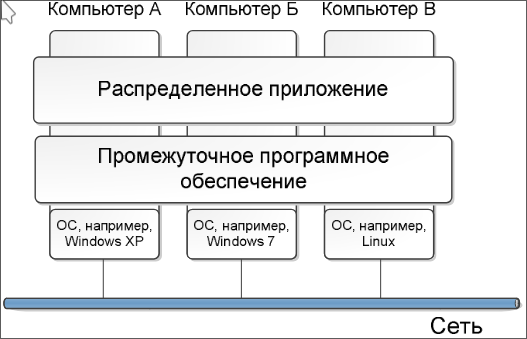
\includegraphics[scale=0.4]{inc/distr-arch.png}
  \caption{Слои программного обеспечения РВС \cite{radchenko2012}}
  \label{fig:distributed-architecture}
\end{figure}

Для того чтобы система выглядела пользователю как единая, применяют следующие
виды прозрачности \cite{radchenko2012}:

\begin{itemize}
    \item \textbf{прозрачность доступа к ресурсам} — пользователи не должны
    замечать различий в способах представления данных и методах доступа;
    \item \textbf{прозрачность размещения} — физическое расположение ресурса не
    влияет на работу пользователя;
    \item \textbf{прозрачность репликации} — наличие нескольких копий ресурса
    скрывается от клиента;
    \item \textbf{прозрачность параллельного доступа} — одновременное
    использование ресурса разными клиентами не должно требовать дополнительной
    координации
    со стороны пользователя;
    \item \textbf{прозрачность отказов} — выход из строя узла или отдельного
    ресурса не должен приводить к потере данных или прекращению работы
    приложений.
\end{itemize}

\subsection{Проблемы согласованности и отказоустойчивости}

Ключевая теоретическая трудность распределённых систем заключается в достижении
согласованного состояния между узлами при наличии сбоев и асинхронности
коммуникаций. Классический результат Фишера—Линч—Патерсона (FLP) показывает
невозможность детерминированного консенсуса в полностью асинхронной системе
даже при наличии одного отказавшего процесса \cite{flp1985}. Этот результат не
делает построение практических систем невозможным, но подчёркивает
необходимость явных инженерных допущений (таймеры, частичная синхронность,
перезапуски) и использования алгоритмов, которые обеспечивают безопасность
(safety) при любой динамике, а живучесть (liveness) — при выполнении
ограниченных условий синхронизации \cite{lynch1996,birman2012}.

Отказоустойчивость в прикладном смысле означает сохранение доступности и
корректности при отказах отдельных узлов и временной недоступности
коммуникационных каналов. Для этого применяются репликация состояния, изоляция
отказов, автоматическое восстановление и предотвращение одновременного
существования нескольких лидеров (split-brain). Наиболее распространённым
конструктом является реплицированная машина состояний: клиентоориентированные
операции записываются в общий лог и детерминированно применяются всеми
репликами в одном и том же порядке, что обеспечивает эквивалентность состояний
\cite{coulouris2012,lynch1996}.

\subsection{Роль алгоритмов консенсуса}

Алгоритм консенсуса описывает работу распределенной системы, которая при наличии
нескольких процессов, начинающих работу с некого начального состояния, переводит
все процессы в одинаковое состояние. Чтобы алгоритм консенсуса был корректным,
должны выполняться следующие условия \cite{petrov}:

\begin{itemize}
    \item Согласованность. Принимаемое протоколом решение должно быть единодушным:
        каждый процесс  выбирает некоторое значение, которое должно быть
        одинаковым для всех процессов.
    \item Действительность. Согласованное значение должно быть предложено одним
        из процессов. Т.е. это не может быть некое произвольное значение.
    \item Окончательность. Согласованность принимает окончательный характер после
        того, как уже не остается процессов, не достигших состояния принятия решения.
\end{itemize}

Алгоритмы консенсуса должны учитывать множество источников недетерминизма:
потери и задержки сообщений, дублирование пакетов, разделение сети (network
partitions), а также отказы узлов как с завершением работы (crash-stop), так и
с восстановлением (crash-recovery) \cite{birman2012, kleppmann2017}. Для
корректной работы требуется наличие \textbf{кворума} — подмножества узлов,
достаточного для принятия решения. Обычно кворумом является простое большинство
($\lceil (N/2) + 1 \rceil$ узлов из $N$), что обеспечивает устойчивость к
отказу меньшей половины кластера.

Особую роль консенсус играет в системах, где требуется \textbf{строгая
согласованность} (linearizability): каждая операция должна выглядеть так, как
будто она выполняется моментально в некоторый момент времени между своим
вызовом и ответом. Без консенсуса реализация таких гарантий невозможна, так как
неконтролируемые сетевые задержки могут привести к рассогласованию состояний.

Современные алгоритмы консенсуса (Paxos, Raft, Zab) используют
похожую модель:
\begin{itemize}
    \item выбор координатора (лидера), который упорядочивает запросы;
    \item протокол подтверждений, гарантирующий, что запись
    добавлена в кворум узлов;
    \item фиксацию (commit), после которой результат становится видим
    всем участникам и может быть применён к состоянию системы.
\end{itemize}

Таким образом, алгоритмы консенсуса служат «системной шиной» для распределённых
приложений, скрывая сложность сетевых сбоев и обеспечивая единообразие работы
кластера. Именно поэтому корректность и эффективность этих алгоритмов
критически важны для построения надёжных распределённых систем.

\subsection{Обоснование выбора алгоритма консенсуса Raft}

Выбор алгоритма консенсуса является ключевым этапом при проектировании
отказоустойчивых распределённых систем. От него напрямую зависят сложность
реализации, удобство сопровождения кода, а также прозрачность поведения системы
для разработчиков и администраторов. Исторически первой широко известной и
формально доказанной реализацией консенсуса был алгоритм Paxos, предложенный
Лампором. Paxos обладает строгими теоретическими гарантиями безопасности и
живучести, но отличается сложной и трудно воспринимаемой спецификацией, что не
раз отмечалось в инженерной литературе и практике промышленной разработки
\cite{lamport2001paxos}. Разработка корректной и полной реализации
Paxos требует значительных усилий и глубокого понимания формальных инвариантов,
что повышает риск ошибок при практическом применении.

Алгоритм Raft был создан как ответ на эту проблему. Его основной целью было
повышение «понимаемости» протокола консенсуса без ущерба для гарантий
корректности. Авторы Raft отмечают, что понимаемость протокола напрямую влияет
на вероятность корректной реализации и снижает риск скрытых ошибок, которые
могут проявиться лишь при сбоях или высокой нагрузке \cite{ongario2014}. Raft
декомпозирует задачу консенсуса на несколько изолированных подпроблем (выбор
лидера, репликация логов, гарантия безопасности логов), что облегчает
рассуждения об инвариантах системы и значительно упрощает обучение
разработчиков.

Дополнительным аргументом в пользу Raft является его популярность и зрелость
реализации в открытых проектах. Сегодня Raft используется во многих
промышленных системах — например, в etcd (сервис конфигурации в Kubernetes),
Consul, TiKV, RethinkDB, Tarantool, что подтверждает его практическую
применимость и широкую проверку в реальных условиях эксплуатации. Благодаря
этому для Raft существует обширная документация, научные статьи, что сокращает
затраты времени на разработку и уменьшает вероятность внедрения ошибок на
ранних этапах.

С точки зрения проектируемой системы, Raft является оптимальным выбором,
так как:
\begin{itemize}
    \item обеспечивает строгую согласованность данных и устойчивость
    к отказу меньшинства узлов;
    \item обладает ясной архитектурой и хорошо описанными сценариями
    поведения при сбоях;
    \item имеет многочисленные реализации и практические рекомендации
    по настройке, что упрощает написание собственной реализации;
    \item подходит для систем с выделенным лидером, где клиентские
    запросы упорядочиваются в единую последовательность,
    что соответствует выбранной архитектуре (узлы Raft управляют
    логом операций и синхронизируют его между собой).
\end{itemize}

Таким образом, Raft предоставляет необходимый баланс между теоретической
строгостью и инженерной простотой, снижая риск некорректной реализации и
ускоряя процесс разработки. Это делает его наиболее подходящим протоколом
консенсуса для решения поставленных в работе задач по обеспечению
отказоустойчивости и согласованности распределённых вычислений.
